\chapter{Realization }

\section{Introduction}

After completing the design phase, we embark on the implementation phase in this chapter. We will begin by presenting the working environment used for development. Then, we will provide an overview of the work accomplished on the developed application. 

\section{Working environment }

\subsection{Hardware environment }

In order to develop our module under the most favorable conditions, we have made available a computer with the following configuration: 
• PC GIGABYTE G5 GE : Intel Core i5-12500H (Up to 4,50 GHz Turbo max, 18 Mo of memory cache, 12-Cores)  with 16GB of RAM
• Operating System: Windows 11 pro 
• Hard disk space: 512 GB SSD

\subsection{Software environment }

In order to develop our application, we have chosen to use the following software environment:

• \textbf{Visual Studio Code:} Visual Studio Code is an extensible code editor developed by Microsoft for Windows, Linux, and macOS. Features include debugging support, syntax highlighting, intelligent code completion, snippets, code refactoring, and integrated Git. 

\subsection{Framework }

        \item \textbf{Angular 14.7.0:} Angular is an open-source client-side framework based on TypeScript, co-led by the Angular team at Google and a community of individuals and corporations. Angular is a complete rewrite of AngularJS, a framework built by the same team. 
        \item \textbf{Spring  Boot 2.7.3:}Spring Boot is a new framework created by the team at Pivotal, designed to simplify the startup and development of new Spring applications. 
\item \textbf{Bootstrap 5.0:} Bootstrap is a collection of tools useful for creating the design (graphics, animations, and page interactions in the browser, etc.) of websites and web applications. It is a set that contains HTML and CSS code, forms, buttons, navigation tools, and other interactive elements, as well as optional JavaScript extensions. 

\subsection{Data Base : MySql  }

\textbf{MySQL} is a relational database management system (RDBMS). It is distributed under a dual GPL and proprietary license. It is one of the most widely used database management software in the world, both by the general public (mainly web applications) and professionals, competing with Oracle, PostgreSQL, and Microsoft SQL Server. 

\section{Work accomplished  }

This section is dedicated to presenting the interfaces of the application developed during this project. 

\subsection{The interfaces of the application  }

•\textbf{ Authentication interface  :}
To log in, the client must enter their email address and password. In the case where the client is not registered, they must create an account. To add a reservation, the user presses the 'add a new reservation button, where they will be redirected to the reservation submission interface. 
 \begin{figure}[H]
   \centering
    %\includegraphics[scale=0.5]{images/trasfvs.jpg}
    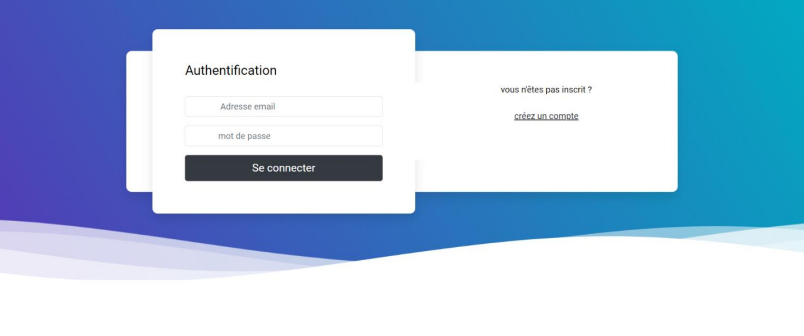
\includegraphics[width=15cm,height=8cm]{images/autint.png}
    \caption{Authentication interface } 
    \label{Authentication interface }
\end{figure}

•\textbf{ Account Creation Interface   :}

Once the client clicks on the 'create an account' link, a form will be displayed for them to create their account by filling out the form with their personal information. 
 \begin{figure}[H]
   \centering
    %\includegraphics[scale=0.5]{images/trasfvs.jpg}
    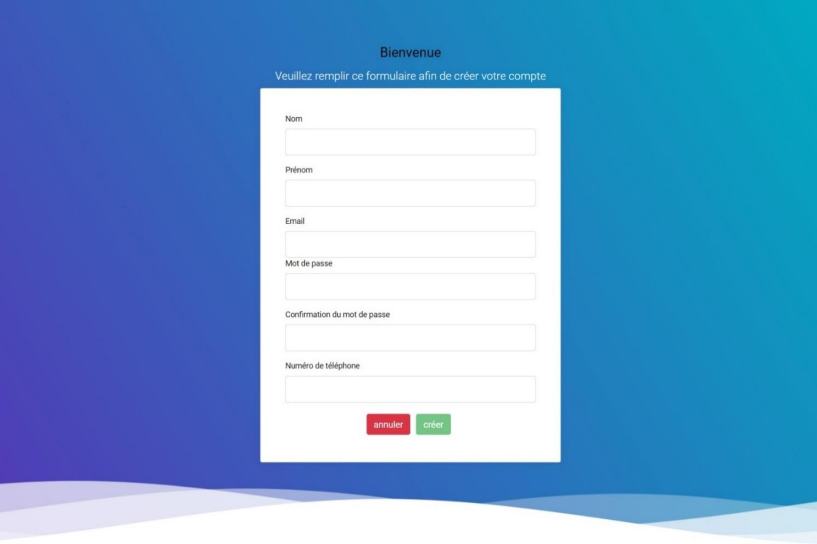
\includegraphics[width=15cm,height=8cm]{images/inscit.png}
    \caption{Account Creation Interface } 
    \label{Account Creation Interface }
\end{figure}


•\textbf{ Admin Interface   :}

\begin{figure}[H]
   \centering
    %\includegraphics[scale=0.5]{images/trasfvs.jpg}
    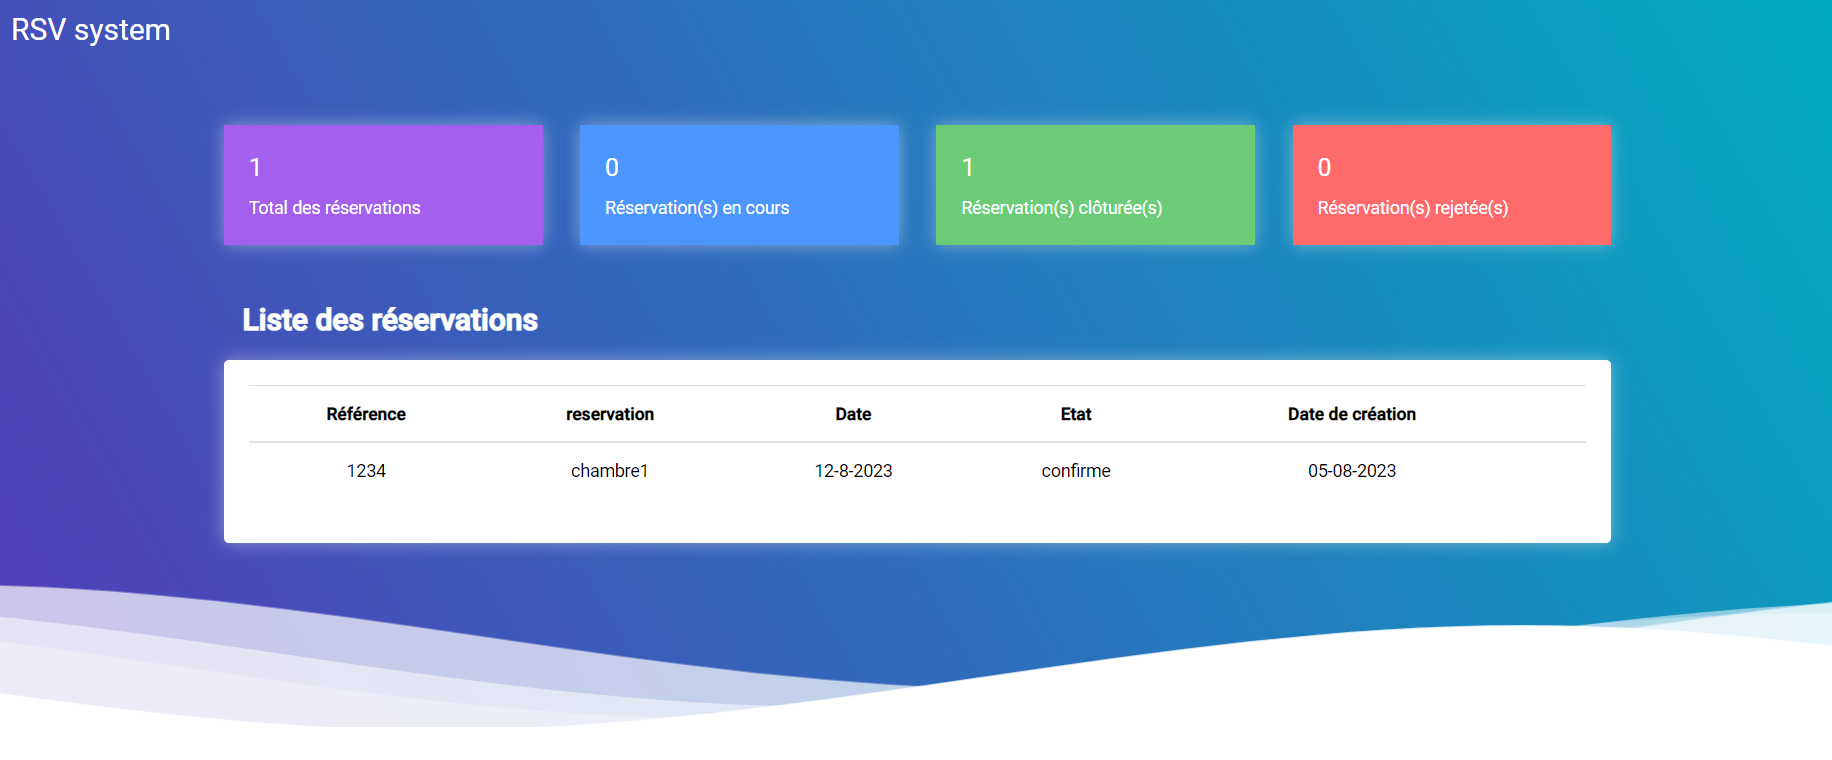
\includegraphics[width=15cm,height=8cm]{images/consint.png}
    \caption{Admin Interface } 
    \label{Admin Interface }
\end{figure}







\section{Conclusion}
This chapter presents the final phase of the project development, which is the implementation phase. Firstly, we defined the working environment and the technologies used, then we presented some screenshots. Finally, we will conclude our report with the consolidated achievements and a general conclusion. 